\chapter{Adversarial Examples}

This chapter is going to focus on Adversarial Examples and how the exploitation of last chapter's network properties can be used to craft such examples. Three methods will be presented along with results found by different studies. Finally, methods for using this adversarial information for regularizing networks will also be shown as a possible solution for making deep neural networks less vulnerable to these kind of attacks.


\section{Fast Gradient Sign}

The Fast Gradient Signed method developed by Goodfellow et al. (2014) has been used as the foundation of many of the experiments in adversarial crafting. The results have led to the hypothesis that DNNs can possibly have linear behavior when in very high dimensional space.  Most inputs were miss-classified not only on Goodfellow et. al \cite{goodfellow2014}  experiments but many other. This shows that adversarial examples are not hard to find. The method consists on using gradient information to generate image noises that changes classification outputs.

$$ C(x + \delta)\approx C(x) + \delta * \nabla C$$

The equation aims into adding noise that emphasizes the pixels in the image with the highest importance, so the resulting perturbation can likely lead to a misclassified result. By using the \textit(sign) function of the gradient, it is assured that the value will grow linearly with the number of the dimensions \cite{goodfellow2014}. The result of many small pixel changes is likely to generate an image with a wrong label in the network output.

$$ C(x + \delta)\approx C(x) + \delta * sign(\nabla C)$$

Billovits et al (2016) used four different categories of adversarials generated by FGSM. True Adversarial are those given a completely different label after being perturbed. Re-Focused adversarial is the method that changes the focus of an image by giving a classification of an object that used to have lower significance while keeping the original object presence. Conaturally Adversarial are those where the new output has some close relation to the miss-classified result (e.g. Dog and Cat). Finally, Benign adversarial hapeens when neural networks misses the top prediction of the original image but the adversarial example gets classified correctly with high confidence \cite{billovits}.

\begin{figure}[!h]
\centering
	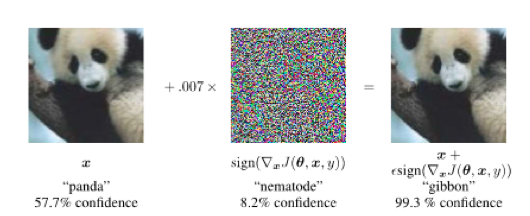
\includegraphics[scale=0.6]{panda.png}
\caption{Adversarial example crafting with fast gradient sign \cite{goodfellow2014}.}
\label{fig:net_change}
\end{figure}

Clearly the method is exploring regions of space that are either completely unexplored or sometimes explorer by classes of different labels.